\section{Introduction}
\label{sec:introduction}

To accompany \TeX{}, Knuth developed \MF{} as a method of ``creating
entire families of fonts from a set of dimensional parameters and
outline descriptions''~\cite{beebe:mf}.  Approximately ten years later,
John Hobby began work on \MP{}\Dash ``a powerful graphics language based
on Knuth's \MF, but with PostScript output and facilities for including
typeset text''~\cite{hobby:user}.  Although several packages (e.g.,
\PiC\TeX, \Xy-pic, and the native \LaTeX{} picture environment to name a
few) are available for creating graphics within \TeX-based documents,
they all rely on \TeX{}.  Since \TeX{} was designed to typeset text, it
seems natural that an external utility should be used to generate
graphics instead.  Furthermore, in the event that the graphics require
typeset text, then the utility should use \TeX{} for this requirement.
This premise is exactly the philosophy of \MP.

Since \MP{} is a programming language, it accommodates data structures
and flow control, and compilation of the \MP{} source code yields \EPS{}
graphics.  These features provide an elegant method for generating
graphics.  \autoref{fig:circles} illustrates how \MP{} can be used
programatically.  The figure is generated by rotating one of the circles
multiple times to obtain the desired \textit{circular chain}.%
\footnote{All graphics in this tutorial (except \autoref{fig:previewer})
  are created with \MP{}, and the source code and any required external
  data files for each of these graphics are embedded as file attachments
  in the electronic \PDF{} version of the article.}

\begin{figure}
  \centering
  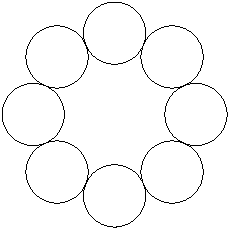
\includegraphics{circles.mps}
  \caption{Rotated circles}
  \label{fig:circles}
  \attach{circles.mp}
\end{figure}

The programming language constructs of \MP{} also deliver a graceful
mechanism for creating animations without having to manually create each
frame of the animation.  The primary advantage of \EPS{} is that it can
be scaled to any resolution without a loss in quality.  It can also be
easily converted to raster formats, e.g.\ Portable Network Graphics
(\PNG) and Joint Photographic Experts Group (\JPEG), et al., or other
vector formats including Portable Document Format (\PDF) and Scalable
Vector Graphics (\SVG), et al.
